\documentclass[10pt]{article}
\usepackage[left=0.4in,right=0.4in,top=0.7in,bottom=0.4in]{geometry}
\usepackage{hyperref}
\usepackage{fancyhdr}
\usepackage{listings}
\usepackage{xcolor}
\usepackage{tocloft}
\usepackage{pdflscape}
\usepackage{multicol}
\usepackage{graphicx}

\renewcommand*{\ttdefault}{pcr}
\renewcommand\cftsecfont{\fontsize{8}{9}\bfseries}
\renewcommand\cftsecpagefont{\fontsize{8}{9}\mdseries}
\renewcommand\cftsubsecfont{\fontsize{5}{6}\mdseries}
\renewcommand\cftsubsecpagefont{\fontsize{5}{6}\mdseries}
\renewcommand\cftsecafterpnum{\vspace{-1ex}}
\renewcommand\cftsubsecafterpnum{\vspace{-1ex}}

\lstdefinestyle{shared}{
    belowcaptionskip=1\baselineskip,
    breaklines=true,
    xleftmargin=\parindent,
    showstringspaces=false,
    basicstyle=\fontsize{5.5}{6}\ttfamily,
}
\lstdefinestyle{cpp}{
	style=shared,
    language=C++,
    keywordstyle=\bfseries\color{green!40!black},
    commentstyle=\itshape\color{red!80!black},
    identifierstyle=\color{blue},
    stringstyle=\color{purple!40!black},
}
\lstdefinestyle{java}{
    style=shared,
    language=Java,
    keywordstyle=\bfseries\color{green!40!black},
    commentstyle=\itshape\color{purple!40!black},
    identifierstyle=\color{blue},
    stringstyle=\color{orange},
}
\lstdefinestyle{py}{
    style=shared,
    language=Python,
    keywordstyle=\bfseries\color{green!40!black},
    commentstyle=\itshape\color{purple!40!black},
    identifierstyle=\color{blue},
    stringstyle=\color{orange},
}
\lstdefinestyle{txt}{
    style=shared,
}
\lstset{escapechar=@}

\pagestyle{fancy}
\fancyhead[L]{INSA Lyon}
\fancyhead[R]{\thepage}
\fancyfoot[C]{}

\fancypagestyle{plain}
{
\fancyhead[L]{INSA Lyon}
\fancyhead[R]{\thepage}
\fancyfoot[C]{}
}

\title{\vspace{-4ex}\Large{INSA Lyon ACM-ICPC Notebook 2018 (Python)}}
\author{}
\date{}

\begin{document}
\begin{landscape}
\begin{multicols}{2}

\maketitle
\vspace{-13ex}
\tableofcontents
\pagestyle{fancy}

\input contents_python.tex

\end{multicols}
\end{landscape}

\centerline{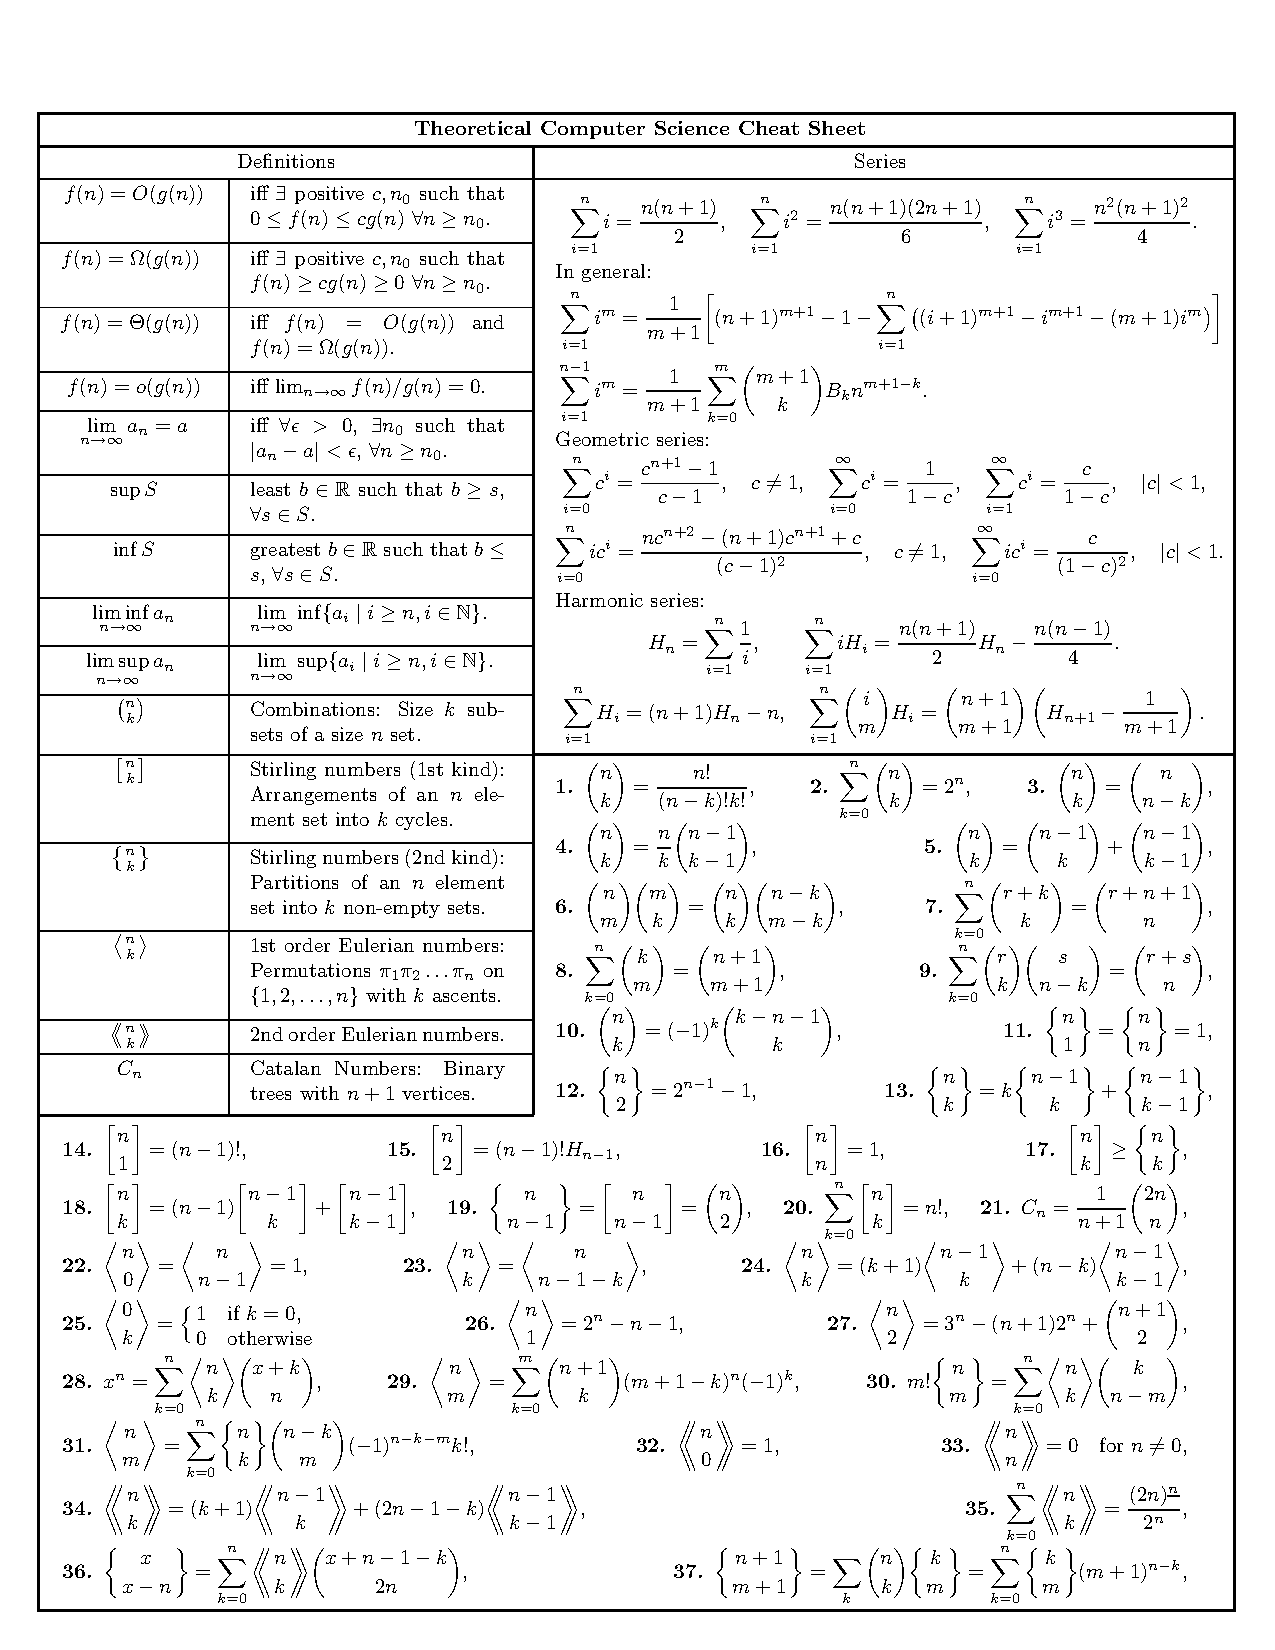
\includegraphics[trim={0 0 0 3cm}, clip, width=\textwidth]{cheatsheet/p01.pdf}}
\centerline{\includegraphics[trim={0 0 0 3cm}, clip, width=\textwidth]{cheatsheet/p02.pdf}}
\centerline{\includegraphics[trim={0 0 0 3cm}, clip, width=\textwidth]{cheatsheet/p03.pdf}}
\centerline{\includegraphics[trim={0 0 0 3cm}, clip, width=\textwidth]{cheatsheet/p04.pdf}}
\centerline{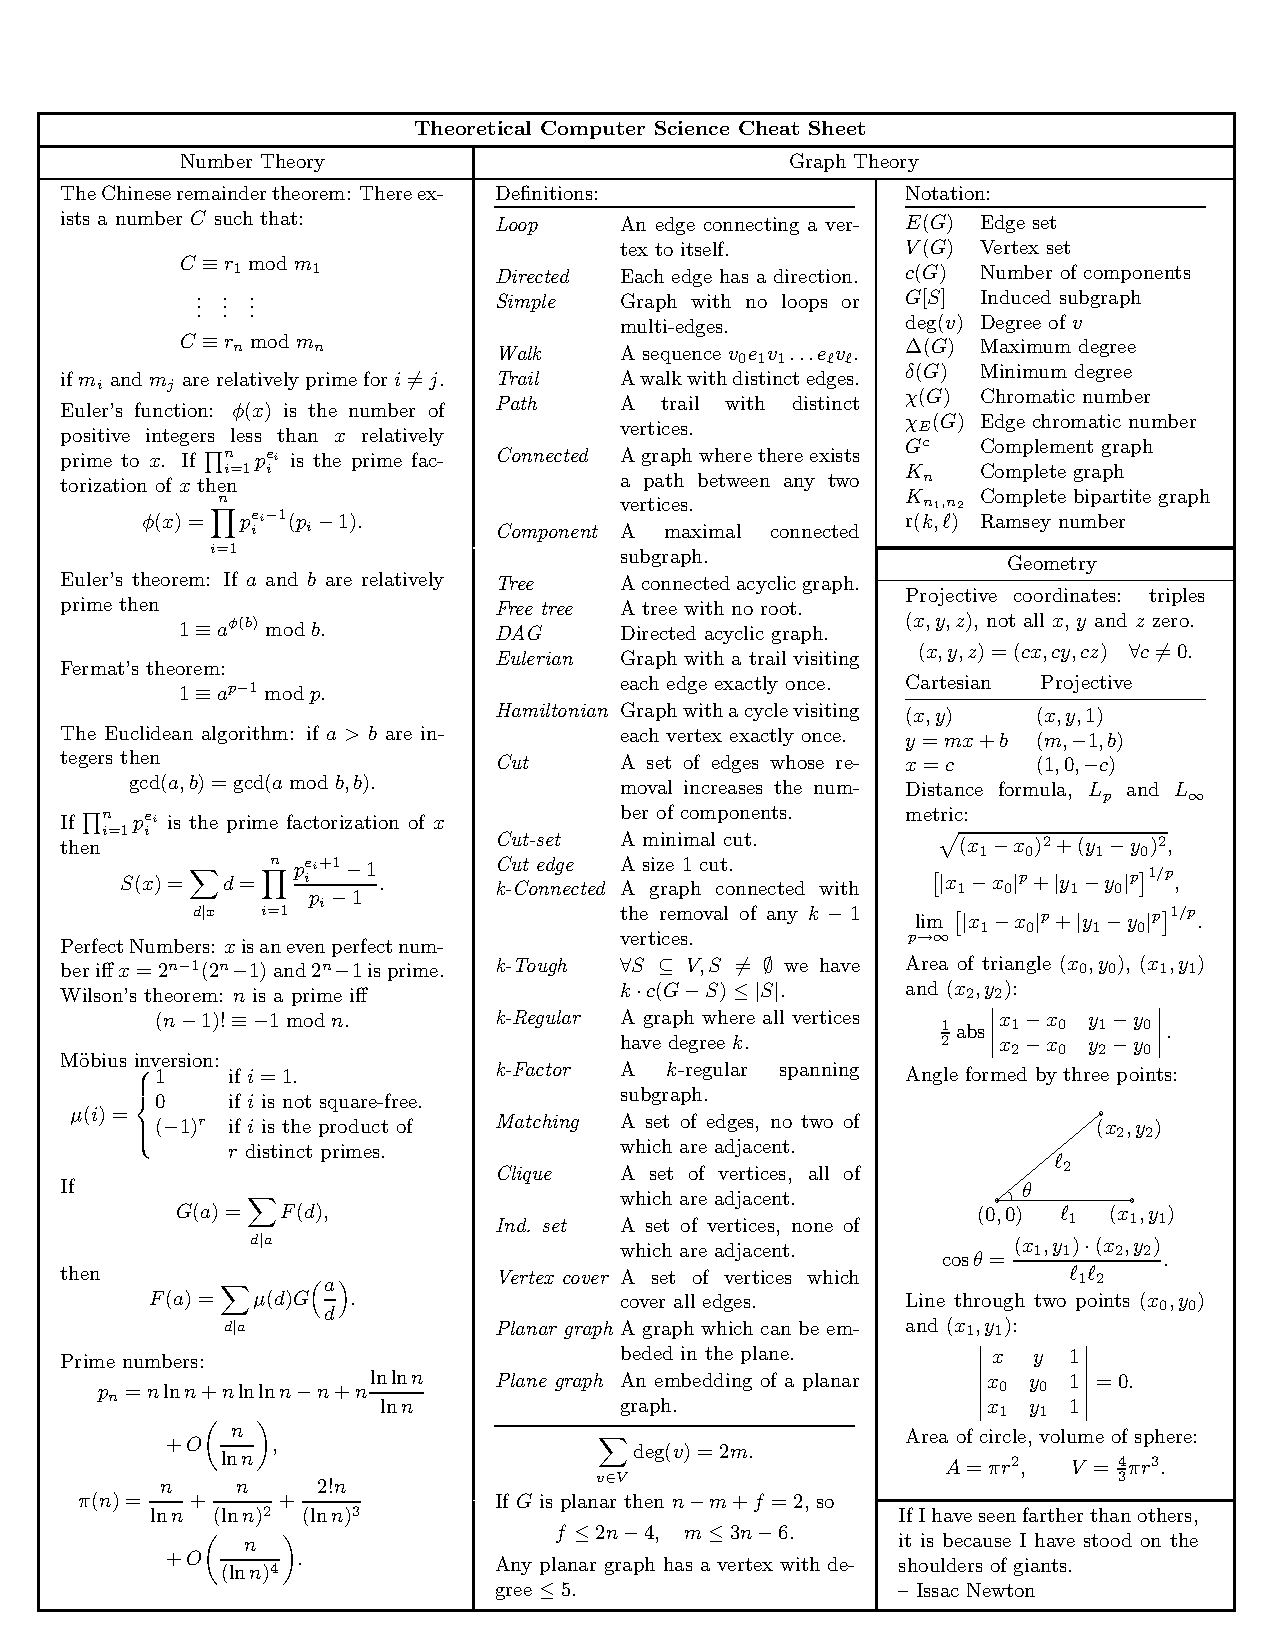
\includegraphics[trim={0 0 0 3cm}, clip, width=\textwidth]{cheatsheet/p05.pdf}}
\centerline{\includegraphics[trim={0 0 0 3cm}, clip, width=\textwidth]{cheatsheet/p06.pdf}}
\centerline{\includegraphics[trim={0 0 0 3cm}, clip, width=\textwidth]{cheatsheet/p07.pdf}}
\centerline{\includegraphics[trim={0 0 0 3cm}, clip, width=\textwidth]{cheatsheet/p08.pdf}}
\centerline{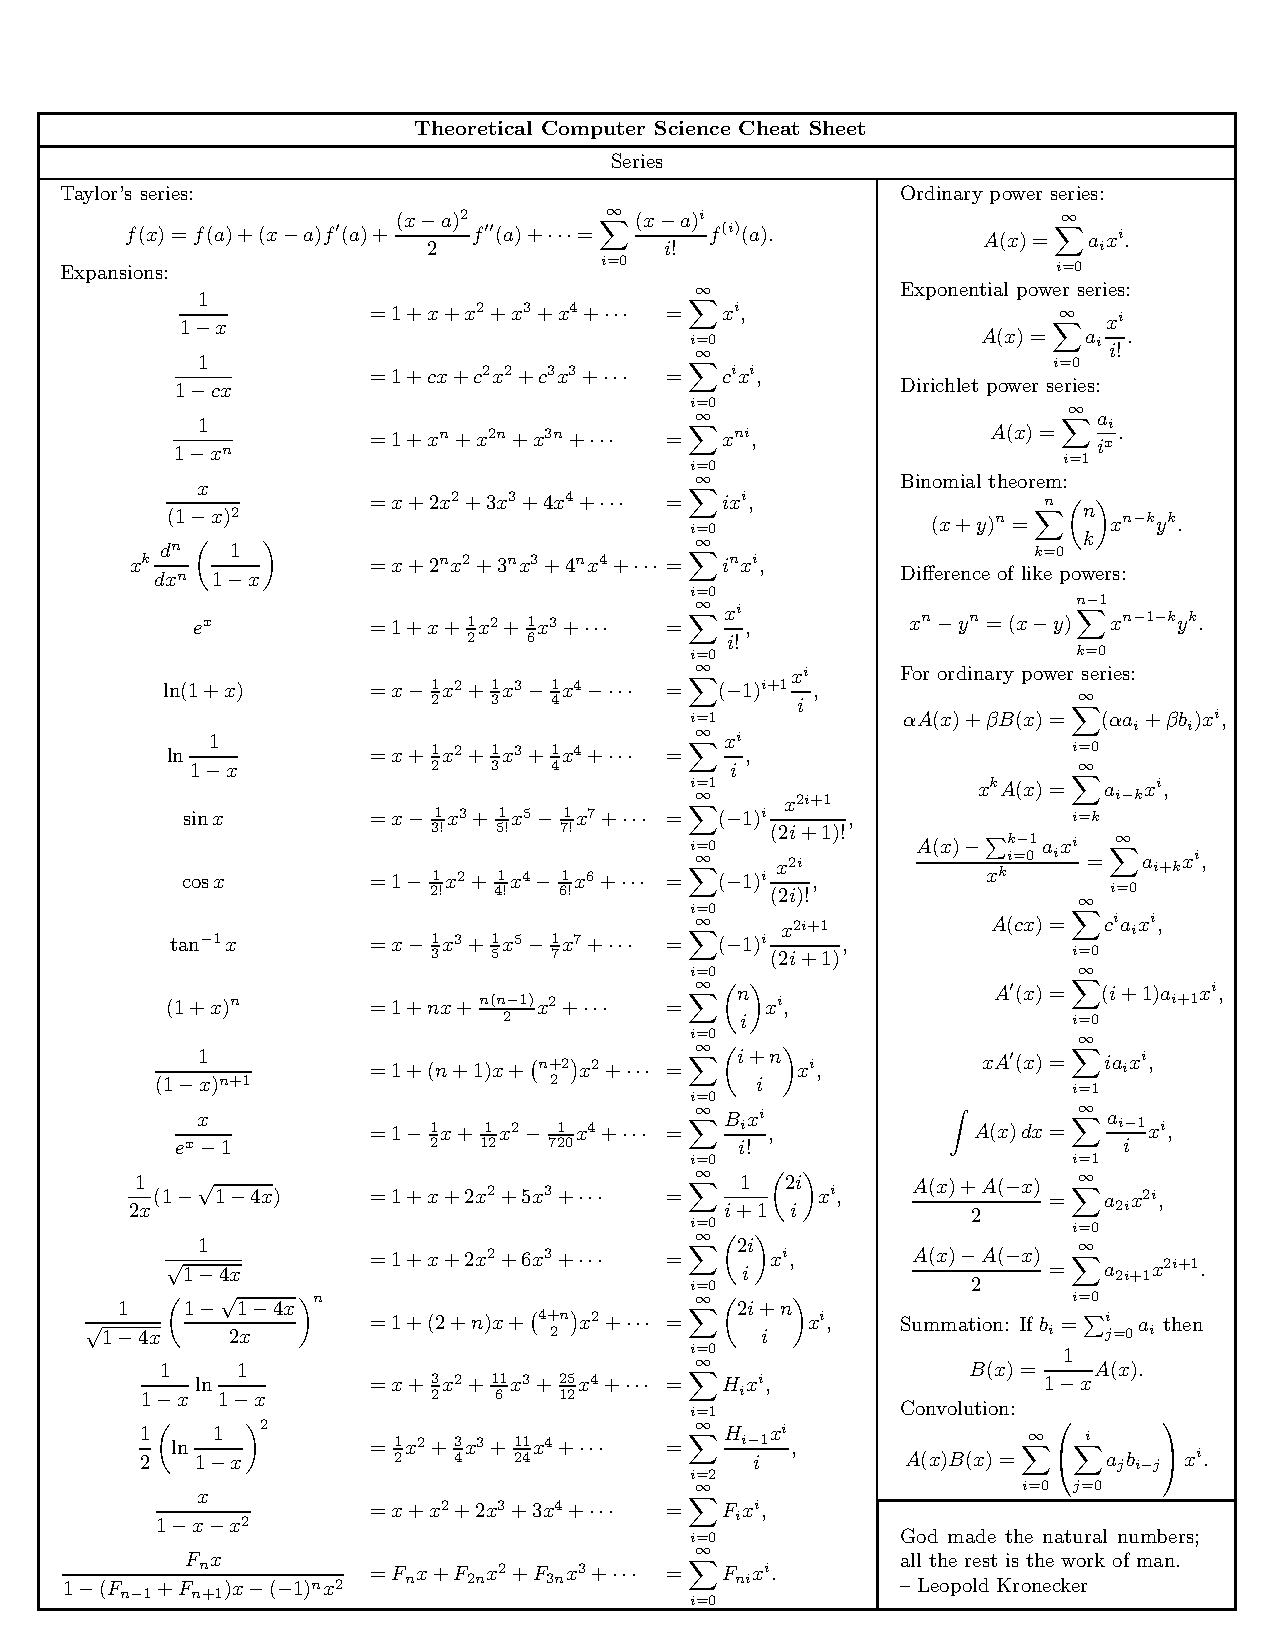
\includegraphics[trim={0 0 0 3cm}, clip, width=\textwidth]{cheatsheet/p09.pdf}}
\centerline{\includegraphics[trim={0 0 0 3cm}, clip, width=\textwidth]{cheatsheet/p10.pdf}}

\newpage
\null
\newpage
\null
\newpage
\null
\end{document}
